\chapter{绪论}\label{ch:绪论}


\section{研究背景及意义}\label{sec:研究背景及意义}

\subsection{研究背景}\label{subsec:研究背景}

自21世纪以来,我国经济迅速发展,大量农村人口涌入城市,使得城市规模越来越大。城市化水平的提高使得城市的交通网络变得异常复杂,也使得对城市交通的管理难度又上了一个台阶。伴随着城市化进程的推进,城市交通问题也逐渐显现出来,其中最突出也是最核心的问题是交通堵塞问题。

交通问题不仅使得资源得不到高效的利用,浪费了道路资源,使得不得不增加一些不必要的支出;也造成了驾驶者经济和精神上的损失,拥挤的道路上车流走走停停,会增加驾驶者的压力,造成心情上的愤怒和烦躁;同时汽车的引擎在堵车路段也必须保持运转,持续燃烧,既是一种资源浪费也会使得城市环境问题变得更加严重;此外由于交通状况不良外加驾驶者情绪不稳定,也更容易产生交通事故。为解决交通拥堵问题,首先需要了解交通堵塞的主要原因,
一般来说主要有以下4个方面:
\begin{enumerate}%有序列表
    \item 区域内有超过交通系统所能承载的负荷量
    \item 资源分配存在区域差异
    \item 历史遗留的道路设计容量不足或设计不当问题
    \item 太多的平面道路交叉或十字路口也会导致交通堵塞
\end{enumerate}


为了解决交通拥堵问题,人们提出过很多方法,在世界经济论坛最新发布的《都市发展的未来行动倡议:大连和张家口建设领军城市战略》汇集了来自世界各地的方法,
以解决污染和其他城市化问题。例如斯德哥尔摩的道路电子收费系统对所有在工作日从上午6:30到下午6:30之间进入市区的驾车人员收费。
只有公交车、出租车、使用绿色燃料的汽车、应急车辆以及利丁厄(Lidingo)岛上的出入车辆可以免费。
巴塞罗那采取了两个措施:一是安装停车场监控摄像头;二是安装交通监控摄像头。停车场的探测器以及视频可以提供是否有停车位的实时数据,这些数据通过城市的无线网络进行传输,把终端用户与市政当局对接起来。伦敦电子行程计划工具提供关于伦敦市内交通路线的即时信息,帮助用户选择不同的交通换乘方式,包括步行、地铁、公交车、轻轨、水上交通和自行车等。小型公共巴士,也被称为小巴,是香港标准巴士路线的补充,服务于一般巴士无法有效到达的区域。小型巴士只有16个座位,其速度更快、效率更高、班次更多,且中途不停靠。丹麦首都一体化的交通系统旨在避免或缓解交通拥堵,该系统整合了三大交通运营商,并实现了企业、政府与其它机构之间的信息互通。一体化的票务系统利用短信服务为乘客提供了便捷的购票服务,让乘客可以方便地了解位置、目的地以及票务信息,同时也为乘客乘坐不同的交通工具以及换乘提供了更大的灵活性和效率。目前来看,主流方法的核心原则都是相同的,即减少单位面积道路内的汽车数量。
一般有以下方案:
\begin{enumerate}%有序列表
    \item 加速道路扩建,提高道路容量
    \item 对车辆的拥有和出行进行限制
    \item 发展公共运输系统
    \item 采取一定的道路收费手段,降低驾驶者的选择率
    \item 实施一些引导居民出行的措施
    \item 构建城市智能交通系统
\end{enumerate}

智能交通系统ITS是为了出行安全方便和提高交通资源的效率,运用实时监测,信息技术,通信技术和计算机控制技术等技术创造的具有人类智慧特征的交通系统。借助ITS可以实现路网信息的集成与共享,通过引 导驾驶者出于利己的考虑,提前绕行或选择其它路段,从而实现宏观调控,达到有效地实现交通流量地分流,避免某些道路成为“热门道路”,而某些道路成为“冷门道路”造成资源地分配不均匀,以充分利用现有道路资源。而在构建城市智能交通系统中,最重要的就是选择最优的路径规划算法,利用路径规划实现从复杂的城市路网中找出最适合用户的路径。

\subsection{研究意义}\label{subsec:研究意义}

对于不同驾驶者的不同需求差异或同一驾驶者不同时间场合下的不同需求差异,或要求距离最短,或要求行程时间最短,或要求行程可靠性最高。以往的交通网络单条最短路问题分析,很大程度上不能适应不同用户的不同需求或同一用户的不同需求等差异化的需求,此外还有可能因网络中路段的故障造成不可达,系统容错性较低。

对于服务提供商(例如,百度地图等)为了提供更好的服务,为出行者提供多条最短路的选择方案,因此出现了多条最短路问题(K Shortest Paths, KSP)。KSP问题输出前K条最短的路径,因此KSP问题相较于最短路问题提供更多的备选方法。KSP是最短路径问题的扩展和变形。

多条最短路问题分析,一方面可以根据驾驶者的特点进行个性化的路线推荐,也能满足因驾驶者临时的特殊需求作出的差异性决策,还能适应因路段施工或路段修复造成路段故障时提供次短路进行推荐,具有一定的系统容错能力和自动修复能力。在具有动态性和不确定性的交通路网中为驾驶者提供具有高可靠性,高鲁棒性的路径导航系统能极大地改善用户体验,所以时间-空间网络下的多条最短路径问题的研究对现实生活有着相当重要的影响和指导作用。


\section{国内外研究现状}\label{sec:国内外研究现状}

根据最短路中源点和汇点的数量和对路径特征的要求,最短路问题可以分为5种类型\cite{lufeng2001}:
\begin{itemize}%无序列表
    \item 一对一节点间的最短路径问题
    \item 一对多节点间的最短路径问题
    \item K条最短路径问题
    \item 实时最短路径问题
    \item 指定必经节点的最短路径问题
\end{itemize}

\subsection{静态最短路问题}\label{subsec:静态最短路问题}

在传统的最短路问题中,城市交通路网中的道路权重一般被认为是常数,而不是关于时间的函数,即静态最短路问题。在这种情况下,可以根据经典的算法,例如Dijkstra算法、Floyd算法、Bellman-Ford算法等进行求解。对于出行者来说,往往会选择成本最小的路径。最短路问题是网络流问题中的基础问题,是指从起点到终点之间选择一条成本最小的路径,可以使用标号设置法、标号修正法或动态规划方法求解。

如果对于驾驶员来说,不仅仅要求选择最短路径,而且具有一些特殊的需求,即附加一些特定的限制条件,例如必须经过某所学校,或避开某些路段,则该问题转变为带有约束的最短路问题。
Dijkstra于1959年提出处理网络中无负权边的静态最短路的Dijkstra算法\cite{dijkstra1959note}。
Jacob等人于1998年放弃了使用双向搜索算法,并认为在实际交通网络中使用该算法是不切实际的\cite{engler1998optimization}。
Zhan和Noon于1996年在美国的10个不同的州构建的大规模路网上对各种最短路算法进行了一个综合的比较\cite{zhan1998shortest}。

\subsection{动态最短路问题}\label{subsec:动态最短路问题}

目前对于静态的最短路径算法的研究已经十分完善,但在实际生活中,网络中的路段阻抗可能会随时发生变化,在很多情况下静态最短路问题的假设条件无法得到满足,传统对路网的静态描述与现实生活中实际遇到的交通网络状况存在较大差距,适用性也极低。随着计算机通信技术的进步和智能交通系统ITS技术的发展,越来越多学者致力于动态最短路问题的研究,一系列针对大规模网络的实时优化算法被提出,动态最短路问题也成为近年来热门研究方向之一。

在最短路问题研究过程中,Chabini首先将A-star算法应用于动态的交通网络中,并指出A-star算法搜索效率与所选取两节点之间最短距离下界之间的关系\cite*{chabini1998discrete}。
Fu和Rilett通过将路段通行时间作为随时间变化的连续的随机函数对路网建模,研究了动态随机最短路问题\cite*{fu1998expected}。
Chabini提出可以使用时空拓展图来表示动态网络,将动态变化的时变行程时间转化为一系列固定费用的时间序列\cite*{chabini1997new}。
邹亮、徐建闽、 朱玲湘首先提出了随机Dijkstra算法,能够快速地从路网中找到最短路径,同时对路网的动态性进行了描述\cite*{邹亮2007算法改进及其在动态最短路径问题中的应用}。
付梦印、李杰等采用道路分层的方法,将大规模的交通道路网络划分为有层次的小网络来降低网络节点的数量,提高运行效率\cite*{付梦印2005基于分层道路网络的新型路径规划算法}。
Nachtigall针对在动态的交通网络中寻找一对一节点的最短路径给出了一个更加高效的AI搜索算法\cite*{nachtigall1995time}。
谭国真和高文等学者通过引入交通路网的时变性来建立最短行程时间模型和K期望最短路模型的形式化描述\cite*{谭国真2003随机时间依赖网络的}。
Kosuch和Lisser在研究动态最短路中假设路段费用已知,但是增加了路段的行程时间延误约束且服从正态分布\cite*{kosuch2010stochastic}。
范巍巍和程琳以路段行程时间服从正态分布为基本前提研究了带有旅行时间方差约束的最短路问题\cite*{范巍巍2007随机路网的最短路径问题研究}。
Chao Sun和 Lin Cheng等学者提出了一个基于距离、行程时间、行程可靠性的多目标用户均衡模型(MUE-TRD)并针对解不唯一的问题提出了最大熵的多目标用户均衡模型(ME-MUE)\cite*{sun2019multi}。

\subsection{k条最短路问题}\label{subsec:k条最短路问题}

Hoffman于1959年首次提出多条最短路问题,即KSP问题\cite*{hoffman1959method}。
Yen采用递推法中偏离路径的思想给出了求解无环的多条最短路的算法\cite*{yen1971finding}。
A. W. Brander和M. C. Sinclair对KSP问题的各种算法进行了一个比较全面的比较分析\cite*{brander1996comparative}。
Shi-Wei LEE和Cheng-Shong Wu 通过将网络种一对一的K条最短路问题转化为最大流和最小费用流问题\cite*{lee1999k}。
Eppstein提出一个时间复杂度为$O(m+nlog(n)+k)$的高效算法用来寻找网络中的K条最短路径\cite*{eppstein1998finding}。


\section{研究内容和技术路线及论文构成}\label{sec:研究内容和技术路线及论文构成}

\subsection{研究内容}\label{subsec:研究内容}
本文的研究任务是在时间-空间网络下完成多条最短路算法的设计,将KSP的方法应用到交通科学中的现实问题。例如,如何利用现有数据为出行者提供多条最短路的选择方案,此外还会进一步拓展,将静态的KSP问题拓展到动态的KSP问题,即时间-空间网络下的多条最短路问题。交通系统中每天获取有大量的数据,可以得到路段的时变旅行时间。加入时间维度,可以更好地利用这些数据,从而为出行者提供更优值的服务。为车辆导航系统的设计提供高可靠性和高鲁棒性的基础,以满足不同驾驶员的个性化需求以及当路段故障时为驾驶者提供最优的备选路径。
本文的研究内容具体如下:
\begin{itemize}%无序列表
    \item \textbf{建立节点拓展的时间-空间网络模型}\\
    在一般的城市道路网络拓扑的基础上,通过对路网的数据结构和路段阻抗函数随时间变化这两个方面进行拓展,引入了交通流的动态性和驾驶者的不同行为对路网的影响,更符合实际交通网络的情况。

    \item \textbf{在时间-空间网络上进行多条最短路分析}\\
    由于在交通网络中,最短路应该默认限制为无环的最短路径。对于存在环路的最短路相当于经过了不必要的冗余路径。在使用A-star算法求解最短路时不会判断最短路是否存在回路,因此使用改进的A-star算法对时间-空间网络进行多条最短路分析,确保最短路中不存在环,从而得到k条最短路径。

    \item \textbf{案例分析和实现k最短路求解程序}\\
    对构造的简单时间-空间网络进行求解,从而证明所建立模型的正确性和本文中提出的算法的有效性,并实现一个可求解时间-空间网络下多条最短路径的应用软件。

    \item \textbf{依据开源平台OpenStreetMap构建城市交通路网并构建路网的时变行程时间}\\
    通过开源平台OpenStreetMap提供的城市路网数据和Uber Movement提供的每条道路的通行速度,借助Python构建城市交通路网并计算时变行程时间(time-dependent travel times)。最终借助开源软件Gephi进行数据可视化展示。
\end{itemize}

\subsection{技术路线}\label{subsec:技术路线}
根据本文的研究目的,论文的研究技术路线图如图\ref{fig:fig1}所示:
\begin{figure}[H] %H为当前位置,!htb为忽略美学标准,htbp为浮动图形
    \centering %图片居中
    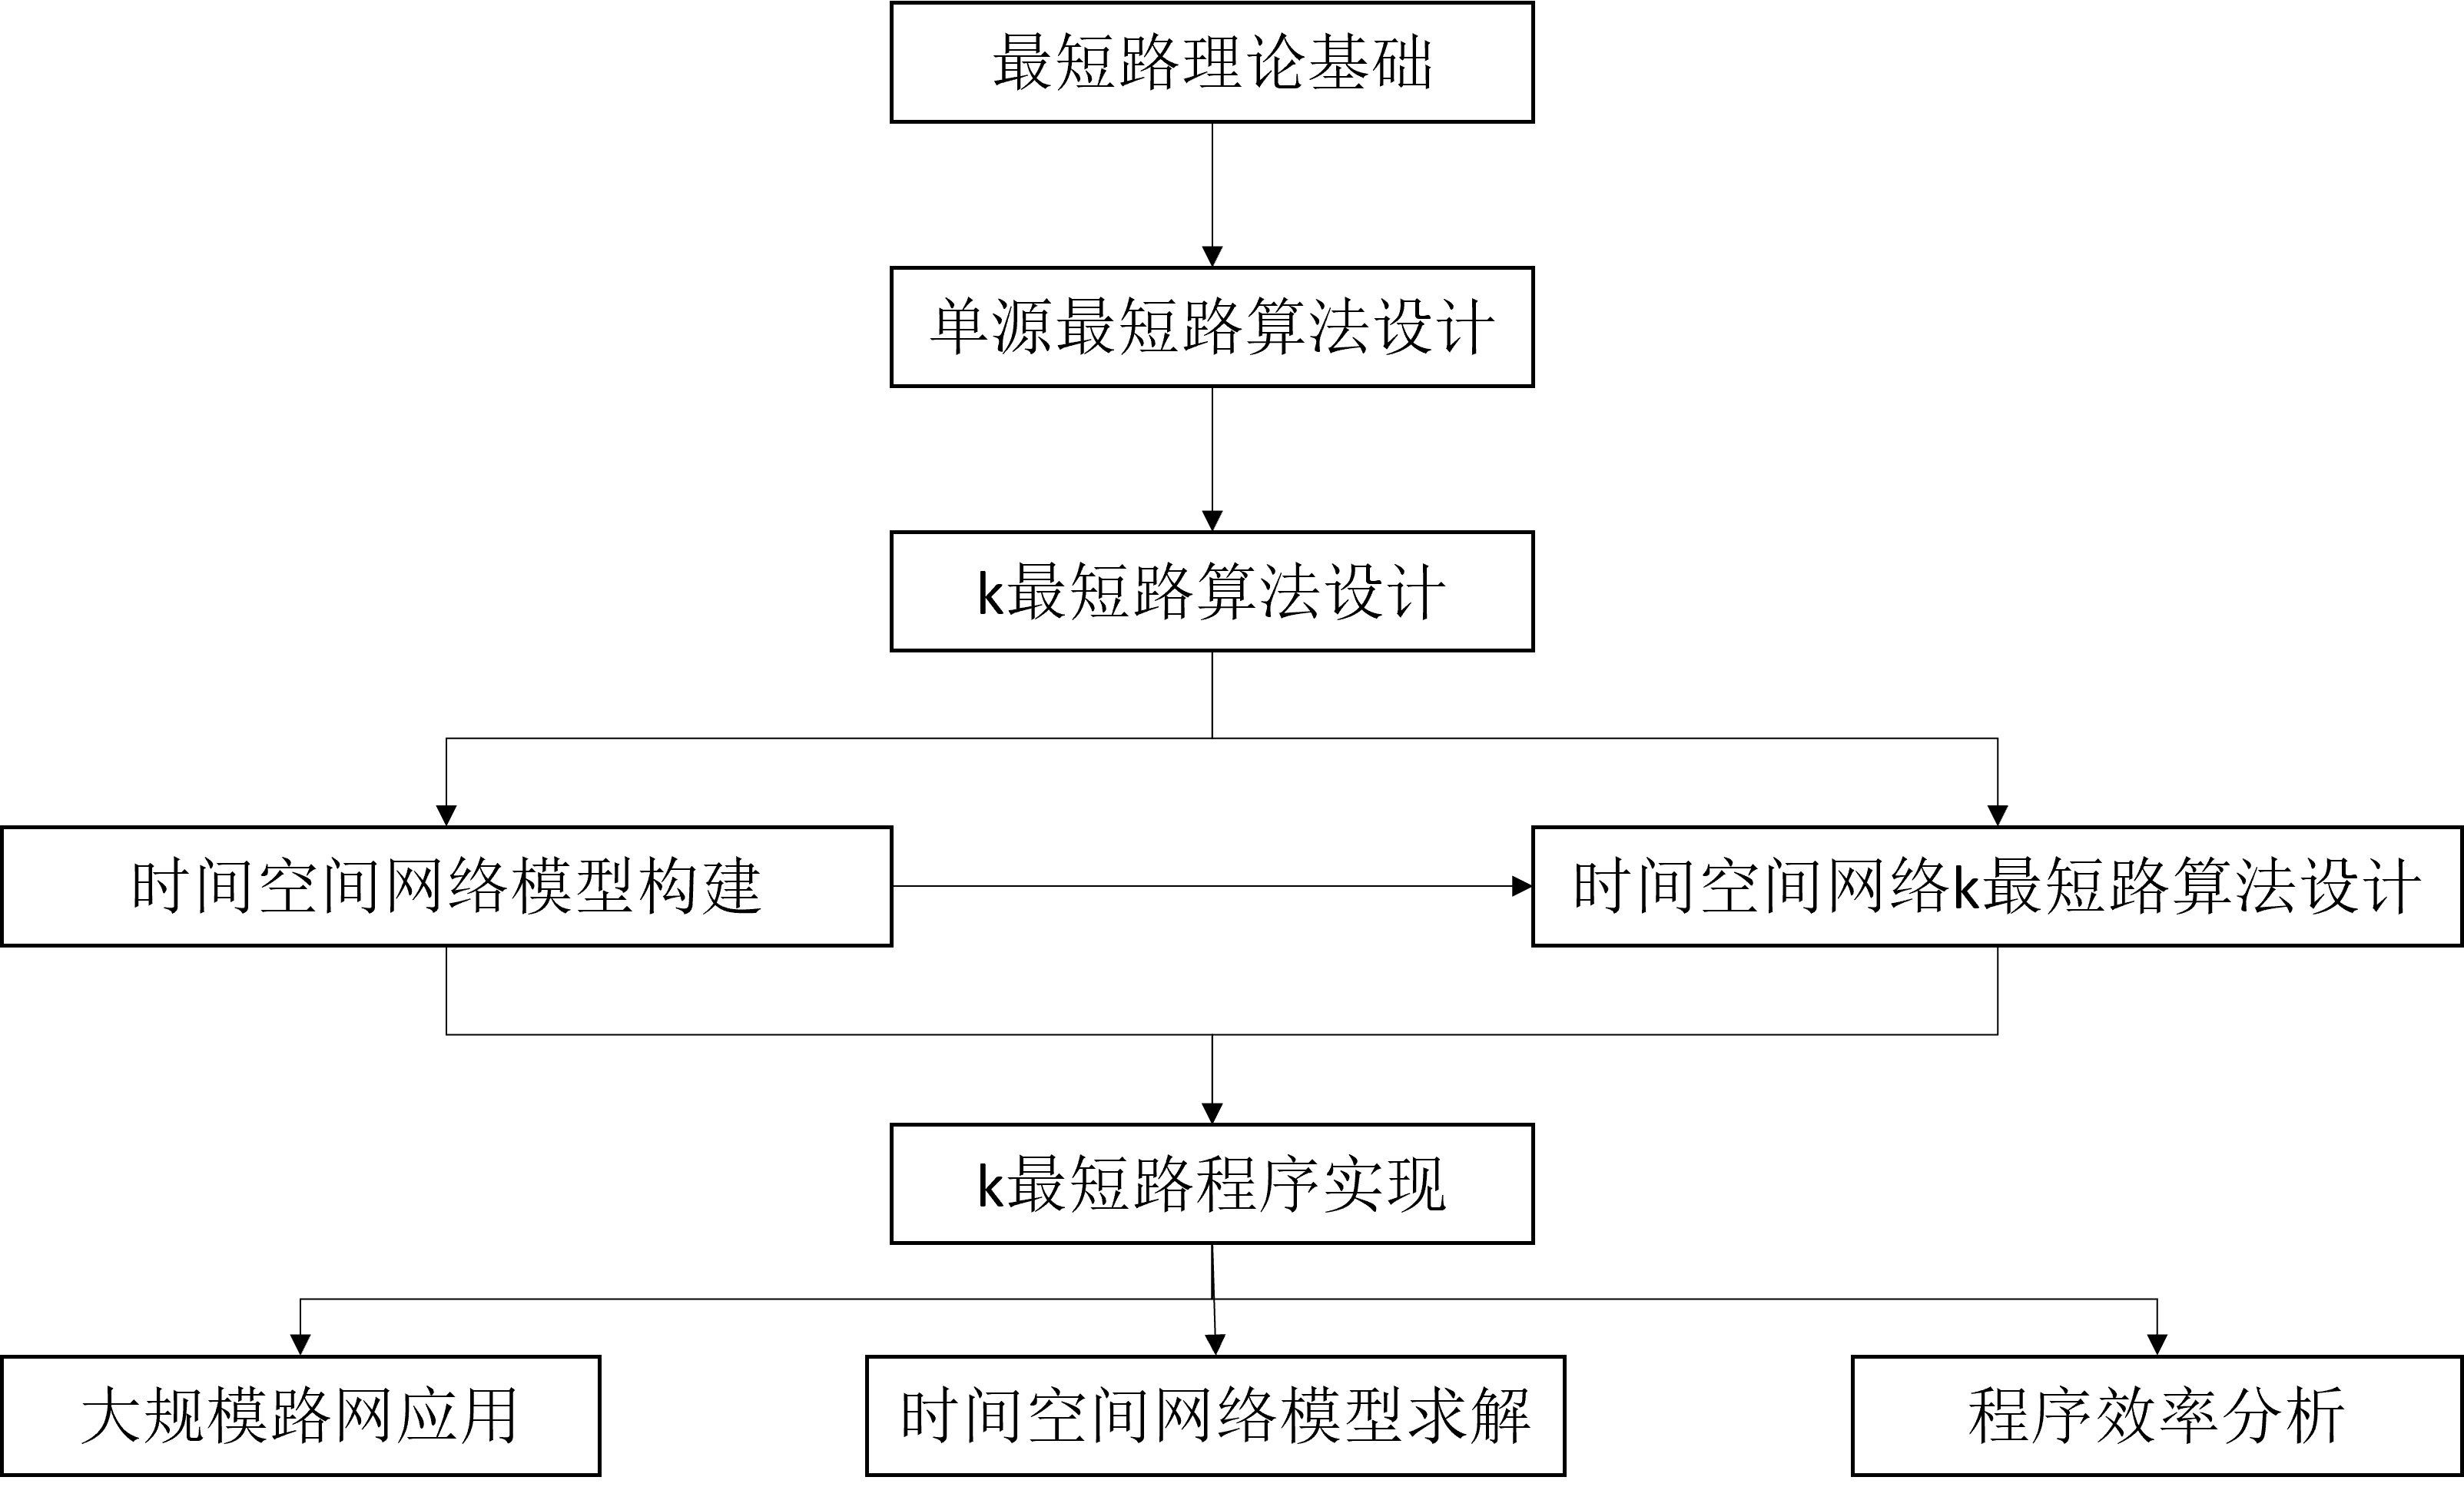
\includegraphics[width=0.7\textwidth]{png/图片1 研究技术路线图} %插入图片,[]中设置图片大小,{}中是图片文件名
    \caption{研究技术路线图} %最终文档中希望显示的图片标题
    \label{fig:fig1} %用于文内引用的标签
\end{figure}

\subsection{论文构成}\label{subsec:论文构成}
论文第1章主要介绍多条最短路在交通领域应用的研究背景和研究意义,目前国内外在相关领域的研究近况以及本文的主要研究内容。


论文第2章主要介绍图论中最短路理论基础,为后面的章节打下基础。


论文第3章结合交通领域的特点,对现有一般网络的拓扑结构进行拓展,并对时间-空间网络进行描述,以便在网络中反映出交通流动态变化的特点。


论文第4章对建立的时间-空间网络模型进行多条最短路算法的设计和求解。


论文第5章通过一个简单的网络案例进行模型的正确性和算法的有效性验证,并通过开源软件进行网络的可视化展示和可达性分析。


论文第6章通过开源平台构建城市交通道路网络并对构建的对象网络进行模拟。

%\nomenclature{PF}{powerful fingers}
%\nomenclature{KF}{kung fu}